\chapter{High-Level Design}

\begin{quotation}
"Software development is not a rational process. It's a process made by people with feelings,
with bodies and with thinking. And by putting all those together I can be a more effective
software enginner."
\end{quotation}
\begin{flushright}
Kent Beck
\end{flushright}

\section{Software Development Methodology}

\begin{center}
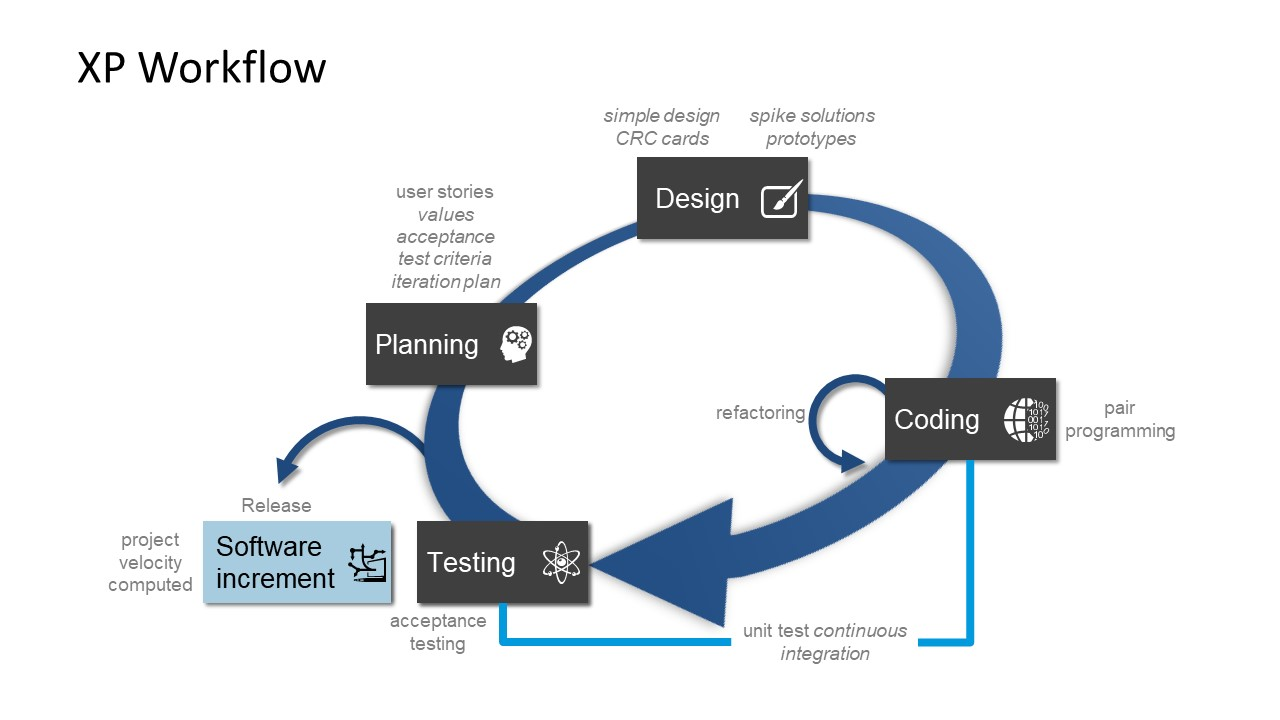
\includegraphics[scale=0.5]{images/xtreme.jpg} 
\captionof{figure}{XP Workflow}
\end{center}


Extreme programming (XP) is a software development methodology which is intended to improve software quality and responsiveness to changing customer requirements. As a type of agile software development, it advocates frequent "releases" in short development cycles, which is intended to improve productivity and introduce checkpoints at which new customer requirements can be adopted.

Other elements of extreme programming include: programming in pairs or doing extensive code review, unit testing of all code, avoiding programming of features until they are actually needed, a flat management structure, code simplicity and clarity, expecting changes in the customer's requirements as time passes and the problem is better understood, and frequent communication with the customer and among programmers.

The methodology takes its name from the idea that the beneficial elements of traditional software engineering practices are taken to "extreme" levels. As an example, code reviews are considered a beneficial practice; taken to the extreme, code can be reviewed continuously, i.e. the practice of pair programming.

\section{Architecture}

\section{RESTful API/End Points}


Each alternative software will be initialized with 0 upvotes and downvotes. These fields will be via \texttt{req.body.<field-name>}. If the \texttt{suggestedBy} field is not specified, then the default value is taken to be "\textsl{anonymous}". If the input syntax does not match this standard, the returned value is a string specifying the error.

\subsection{\texttt{GET Requests}}

\begin{itemize}

\item{\texttt{'GET' /}}

Home Page

\item{\texttt{'GET' /api/login/me}}

Used to query the database for user information. A token needs to be sent in the header of the request which shall then be verified. On successful varification, usernmae, firstName and lastName are returned in response. Otherwise a 400 eror is raised.

\item{\texttt{'GET' /api/proprietary}}

Returns an array of all proprietary softwares as an array of objects.

\item{\texttt{'GET' /api/alternatives}}

Return an array of the top 10 alternatives (Free Softwares) as an array of objects containing the name, license and upVotes for the softwares in decreasing order.

\item{\texttt{'GET' /api/alternatives/<id>}}

Returns the alternatives for the proprietary software specified by id. id has to be passed as a in the url.

\end{itemize}

\subsection{\texttt{POST Requests}}

\begin{itemize}

\item{\texttt{'POST' /api/alternatives}}

To add a new alternative to the free softwares. The body of the request contains the following fields:

\begin{itemize}
\item \texttt{name}: The name of the software
\item \texttt{shortDescription}: A one line description of it
\item \texttt{handle}: A single keyword which will be used to assign it as an alternative
\item \texttt{license}: The software's license
\item \texttt{suggestedBy}: The username of the user who proposed this alternative
\end{itemize}

\item{\texttt{'POST' /api/proprietary/}}

This will add a new proprietary software. Similar to adding alternative softwares, here also the request body must contain the following fields:
\begin{itemize}
\item \texttt{name}: name of the proprietary software
\item \texttt{shortDescription}: One line description of the software
\item \texttt{tags}: A string array consisting of strings that will be matched against the handle of the alternative softwares to verify it is an alternative
\item \texttt{requestedBy}: Username of the user who put up this proprietary software request
\end{itemize}

If the \texttt{requestedBy} field is not specified, then the default value is taken to be "\textsl{anonymous}". If the input syntax does not match this standard, the returned value is a string specifying the error.



\item{\texttt{'POST' /api/proprietary/}}

Used to search for proprietary softwares. The pattern will be used as a regular expression to search for proprietary softwares. Pass the search string the user enters to this endpoint. Returns an array of objects corresponding to the proprietary softwares matching the given search string. The string will be passed as a property 'search' inside the \texttt{req.body}.


\item{\texttt{'POST' /api/alternatives/license/}}

Used to search alternative softwares to check their license. Returns an array of objects containing the name of the alternatives matching the search property of the req.body object. The matching is done as regExp matching ignoring case.


\item{\texttt{'POST' /api/proprietary/search/}}

Used to search proprietary softwares. Returns an array of objects containing the name and shortDescription of the proprietary softwares matching the search property of the req.bodyobject. The matching is done as regExp matching ignoring case.


\item{\texttt{'POST' /api/signup}}

Used to sign-up a user onto the application. It takes user credentials in the request's body and then validates for correcteness. If validation passes, the user is stored onto the database and automatically logged in. Additionally, a json web token is sent for future use. If the validation fails, the user is prompted with appropriate error message.


\item{\texttt{'POST' /api/login}}

Used to log-in a user onto the application. There are two ways of doing it : 

\begin{enumerate}
\item \textbf{Through log-in credentials} : This method involves user sending in his uername/email and password. On successful validation of the credentials, user is logged onto the system as well as a json web token is sent for future use(session handling).

\item \textbf{Through json web token} : If a user queries with a valid json web token, he is logged onto the system after varifying the token's authenticity. Otherwise an \texttt{invalid-token} error is raised.
\end{enumerate}

\end{itemize}


\subsection{\texttt{PUT Requests}}

\begin{itemize}

\item{\texttt{'PUT' /api/alternatives/upvote/<id>}}
This will increase number of upvotes for the given alternative software specified by id by 1. The id has to be passed as a parameter in the url.


\item{\texttt{'PUT' /api/alternatives/unupvote/<id>}}
Will reduce the number of upvotes for the given alternative software specified by id by 1. The id has to be passed as a parameter in the url. Automatically checks if the upvotes is already at 0, doesn’t do anything.


\item{\texttt{'PUT' /api/alternatives/downvote/<id>}}
This will increase number of downvotes for the given alternative software specified by id by 1. The id has to be passed as a parameter in the url.


\item{\texttt{'PUT' /api/alternatives/undownvote/<id>}}
Will reduce the number of downvotes for the given alternative software specified by id by 1. The id has to be passed as a parameter in the url. Automatically checks if the upvotes is already at 0, doesn’t do anything.

\end{itemize}



